% Options for packages loaded elsewhere
\PassOptionsToPackage{unicode}{hyperref}
\PassOptionsToPackage{hyphens}{url}
\PassOptionsToPackage{dvipsnames,svgnames,x11names}{xcolor}
%
\documentclass[
  12pt]{article}

\usepackage{amsmath,amssymb}
\usepackage{lmodern}
\usepackage{iftex}
\ifPDFTeX
  \usepackage[T1]{fontenc}
  \usepackage[utf8]{inputenc}
  \usepackage{textcomp} % provide euro and other symbols
\else % if luatex or xetex
  \usepackage{unicode-math}
  \defaultfontfeatures{Scale=MatchLowercase}
  \defaultfontfeatures[\rmfamily]{Ligatures=TeX,Scale=1}
\fi
% Use upquote if available, for straight quotes in verbatim environments
\IfFileExists{upquote.sty}{\usepackage{upquote}}{}
\IfFileExists{microtype.sty}{% use microtype if available
  \usepackage[]{microtype}
  \UseMicrotypeSet[protrusion]{basicmath} % disable protrusion for tt fonts
}{}
\makeatletter
\@ifundefined{KOMAClassName}{% if non-KOMA class
  \IfFileExists{parskip.sty}{%
    \usepackage{parskip}
  }{% else
    \setlength{\parindent}{0pt}
    \setlength{\parskip}{6pt plus 2pt minus 1pt}}
}{% if KOMA class
  \KOMAoptions{parskip=half}}
\makeatother
\usepackage{xcolor}
\setlength{\emergencystretch}{3em} % prevent overfull lines
\setcounter{secnumdepth}{5}
% Make \paragraph and \subparagraph free-standing
\ifx\paragraph\undefined\else
  \let\oldparagraph\paragraph
  \renewcommand{\paragraph}[1]{\oldparagraph{#1}\mbox{}}
\fi
\ifx\subparagraph\undefined\else
  \let\oldsubparagraph\subparagraph
  \renewcommand{\subparagraph}[1]{\oldsubparagraph{#1}\mbox{}}
\fi

\usepackage{color}
\usepackage{fancyvrb}
\newcommand{\VerbBar}{|}
\newcommand{\VERB}{\Verb[commandchars=\\\{\}]}
\DefineVerbatimEnvironment{Highlighting}{Verbatim}{commandchars=\\\{\}}
% Add ',fontsize=\small' for more characters per line
\usepackage{framed}
\definecolor{shadecolor}{RGB}{241,243,245}
\newenvironment{Shaded}{\begin{snugshade}}{\end{snugshade}}
\newcommand{\AlertTok}[1]{\textcolor[rgb]{0.68,0.00,0.00}{#1}}
\newcommand{\AnnotationTok}[1]{\textcolor[rgb]{0.37,0.37,0.37}{#1}}
\newcommand{\AttributeTok}[1]{\textcolor[rgb]{0.40,0.45,0.13}{#1}}
\newcommand{\BaseNTok}[1]{\textcolor[rgb]{0.68,0.00,0.00}{#1}}
\newcommand{\BuiltInTok}[1]{\textcolor[rgb]{0.00,0.23,0.31}{#1}}
\newcommand{\CharTok}[1]{\textcolor[rgb]{0.13,0.47,0.30}{#1}}
\newcommand{\CommentTok}[1]{\textcolor[rgb]{0.37,0.37,0.37}{#1}}
\newcommand{\CommentVarTok}[1]{\textcolor[rgb]{0.37,0.37,0.37}{\textit{#1}}}
\newcommand{\ConstantTok}[1]{\textcolor[rgb]{0.56,0.35,0.01}{#1}}
\newcommand{\ControlFlowTok}[1]{\textcolor[rgb]{0.00,0.23,0.31}{#1}}
\newcommand{\DataTypeTok}[1]{\textcolor[rgb]{0.68,0.00,0.00}{#1}}
\newcommand{\DecValTok}[1]{\textcolor[rgb]{0.68,0.00,0.00}{#1}}
\newcommand{\DocumentationTok}[1]{\textcolor[rgb]{0.37,0.37,0.37}{\textit{#1}}}
\newcommand{\ErrorTok}[1]{\textcolor[rgb]{0.68,0.00,0.00}{#1}}
\newcommand{\ExtensionTok}[1]{\textcolor[rgb]{0.00,0.23,0.31}{#1}}
\newcommand{\FloatTok}[1]{\textcolor[rgb]{0.68,0.00,0.00}{#1}}
\newcommand{\FunctionTok}[1]{\textcolor[rgb]{0.28,0.35,0.67}{#1}}
\newcommand{\ImportTok}[1]{\textcolor[rgb]{0.00,0.46,0.62}{#1}}
\newcommand{\InformationTok}[1]{\textcolor[rgb]{0.37,0.37,0.37}{#1}}
\newcommand{\KeywordTok}[1]{\textcolor[rgb]{0.00,0.23,0.31}{#1}}
\newcommand{\NormalTok}[1]{\textcolor[rgb]{0.00,0.23,0.31}{#1}}
\newcommand{\OperatorTok}[1]{\textcolor[rgb]{0.37,0.37,0.37}{#1}}
\newcommand{\OtherTok}[1]{\textcolor[rgb]{0.00,0.23,0.31}{#1}}
\newcommand{\PreprocessorTok}[1]{\textcolor[rgb]{0.68,0.00,0.00}{#1}}
\newcommand{\RegionMarkerTok}[1]{\textcolor[rgb]{0.00,0.23,0.31}{#1}}
\newcommand{\SpecialCharTok}[1]{\textcolor[rgb]{0.37,0.37,0.37}{#1}}
\newcommand{\SpecialStringTok}[1]{\textcolor[rgb]{0.13,0.47,0.30}{#1}}
\newcommand{\StringTok}[1]{\textcolor[rgb]{0.13,0.47,0.30}{#1}}
\newcommand{\VariableTok}[1]{\textcolor[rgb]{0.07,0.07,0.07}{#1}}
\newcommand{\VerbatimStringTok}[1]{\textcolor[rgb]{0.13,0.47,0.30}{#1}}
\newcommand{\WarningTok}[1]{\textcolor[rgb]{0.37,0.37,0.37}{\textit{#1}}}

\providecommand{\tightlist}{%
  \setlength{\itemsep}{0pt}\setlength{\parskip}{0pt}}\usepackage{longtable,booktabs,array}
\usepackage{calc} % for calculating minipage widths
% Correct order of tables after \paragraph or \subparagraph
\usepackage{etoolbox}
\makeatletter
\patchcmd\longtable{\par}{\if@noskipsec\mbox{}\fi\par}{}{}
\makeatother
% Allow footnotes in longtable head/foot
\IfFileExists{footnotehyper.sty}{\usepackage{footnotehyper}}{\usepackage{footnote}}
\makesavenoteenv{longtable}
\usepackage{graphicx}
\makeatletter
\def\maxwidth{\ifdim\Gin@nat@width>\linewidth\linewidth\else\Gin@nat@width\fi}
\def\maxheight{\ifdim\Gin@nat@height>\textheight\textheight\else\Gin@nat@height\fi}
\makeatother
% Scale images if necessary, so that they will not overflow the page
% margins by default, and it is still possible to overwrite the defaults
% using explicit options in \includegraphics[width, height, ...]{}
\setkeys{Gin}{width=\maxwidth,height=\maxheight,keepaspectratio}
% Set default figure placement to htbp
\makeatletter
\def\fps@figure{htbp}
\makeatother

\addtolength{\oddsidemargin}{-.5in}%
\addtolength{\evensidemargin}{-1in}%
\addtolength{\textwidth}{1in}%
\addtolength{\textheight}{1.7in}%
\addtolength{\topmargin}{-1in}%
\usepackage{amsmath}
\usepackage{booktabs}
\usepackage{caption}
\usepackage{longtable}
\makeatletter
\makeatother
\makeatletter
\makeatother
\makeatletter
\@ifpackageloaded{caption}{}{\usepackage{caption}}
\AtBeginDocument{%
\ifdefined\contentsname
  \renewcommand*\contentsname{Table of contents}
\else
  \newcommand\contentsname{Table of contents}
\fi
\ifdefined\listfigurename
  \renewcommand*\listfigurename{List of Figures}
\else
  \newcommand\listfigurename{List of Figures}
\fi
\ifdefined\listtablename
  \renewcommand*\listtablename{List of Tables}
\else
  \newcommand\listtablename{List of Tables}
\fi
\ifdefined\figurename
  \renewcommand*\figurename{Figure}
\else
  \newcommand\figurename{Figure}
\fi
\ifdefined\tablename
  \renewcommand*\tablename{Table}
\else
  \newcommand\tablename{Table}
\fi
}
\@ifpackageloaded{float}{}{\usepackage{float}}
\floatstyle{ruled}
\@ifundefined{c@chapter}{\newfloat{codelisting}{h}{lop}}{\newfloat{codelisting}{h}{lop}[chapter]}
\floatname{codelisting}{Listing}
\newcommand*\listoflistings{\listof{codelisting}{List of Listings}}
\makeatother
\makeatletter
\@ifpackageloaded{caption}{}{\usepackage{caption}}
\@ifpackageloaded{subcaption}{}{\usepackage{subcaption}}
\makeatother
\makeatletter
\@ifpackageloaded{tcolorbox}{}{\usepackage[many]{tcolorbox}}
\makeatother
\makeatletter
\@ifundefined{shadecolor}{\definecolor{shadecolor}{rgb}{.97, .97, .97}}
\makeatother
\makeatletter
\makeatother
\ifLuaTeX
  \usepackage{selnolig}  % disable illegal ligatures
\fi
\usepackage[]{natbib}
\bibliographystyle{agsm}
\IfFileExists{bookmark.sty}{\usepackage{bookmark}}{\usepackage{hyperref}}
\IfFileExists{xurl.sty}{\usepackage{xurl}}{} % add URL line breaks if available
\urlstyle{same} % disable monospaced font for URLs
\hypersetup{
  pdftitle={Assessing graduates readiness for job market skills},
  pdfauthor={Zahid Asghar},
  pdfkeywords={Future jobs, Future of Universities, Time vs Learning
goals},
  colorlinks=true,
  linkcolor={blue},
  filecolor={Maroon},
  citecolor={Blue},
  urlcolor={Blue},
  pdfcreator={LaTeX via pandoc}}


\begin{document}


\def\spacingset#1{\renewcommand{\baselinestretch}%
{#1}\small\normalsize} \spacingset{1}


%%%%%%%%%%%%%%%%%%%%%%%%%%%%%%%%%%%%%%%%%%%%%%%%%%%%%%%%%%%%%%%%%%%%%%%%%%%%%%

\date{November 29, 2022}
\title{\bf Assessing graduates readiness for job market skills}
\author{
Zahid Asghar\thanks{The author gratefully acknowledges Pakistan Society
of Development Economics to provide opportunity to provide an
opportunity to present this work at 36th AGM, Quetta.}\\
School of Economics, Quaid-i-Azam University\\
}
\maketitle

\bigskip
\bigskip
\begin{abstract}
Employers are facing a great chasm between skills currently prevailing,
and skills required. On the other hand, there is an overwhelming youth
seeking jobs. In a very challenging environment where skills for jobs of
today and tomorrow are changing rapidly, it is important to assess our
graduates' readiness for jobs with skills in demand in the market. This
study is explores how familiar our graduates with challenges and major
disruptions in jobs market by digital revolution, artificial
intelligence , machine learning among many other developments. I also
assess graduates'\,' readiness for jobs of today and tomorrow also on a
certain skill set highlighted by World Economic Forum 2020 Opinion
survey conducted from recently graduated/last year university four year
degree program students and MPhil/PhD students indicate element of
worriness, lack of awareness of future uncertainties and relatively more
focus on hard work than soft skills. Absence of career counseling and
being in the right discipline are perceived as some of the main reasons
for many graduates' poor academic performance and under-equipment with
right set of skills. On the positive side, large number of students
reported as hard working and punctual which implies that better
mentoring and exposure to our youth may equip them with right skills and
they may avail right openings and excel. There is need that universities
adapt a new learning eco-system for producing graduates to be successful
in the job market.
\end{abstract}

\noindent%
{\it Keywords:} Future jobs, Future of Universities, Time vs Learning
goals
\vfill

\newpage
\spacingset{1.9} % DON'T change the spacing!
\ifdefined\Shaded\renewenvironment{Shaded}{\begin{tcolorbox}[sharp corners, borderline west={3pt}{0pt}{shadecolor}, boxrule=0pt, breakable, enhanced, frame hidden, interior hidden]}{\end{tcolorbox}}\fi

\hypertarget{sec-intro}{%
\section{Introduction}\label{sec-intro}}

Pakistan has huge youth bulge and economic growth is not sufficient to
create opportunities to absorb this burgeoning youth. On the positive
side, digital revolution, gig economy and Silicon Valley era have opened
jobs which are global in nature. But is our work force ready to benefit
from such opportunities which exist both at national and global level?
What sort of skilling and reskilling may help our burgeoning young
population and labor force to unlock their potential? How and where
long-term investment by the institutions in skilling and reskilling of
youth and working population should be made? All this demands deep
introspection and integrated thinking as finding answers to these
questions and devising a mechanism, accordingly, will help our youth to
excel besides having healthy economy. Two decades back, occupation
specific skills and high academic qualifications were sufficient for
graduates to enter into the workforce. However, due to digital
revolution, the selection criteria for a sizeable portion of employees
in the workforce began to change \citet{assessme2015} . Firms, companies
and entrepreneurs are placing increasing value on graduates being work
ready. Employers invest little in workers as they may hire someone for a
short term. In gig-economy, one is not looking for hiring of young
graduates as their precious future commodity, therefore, they prefer to
hire graduates well equipped with skills instead of hiring and investing
to make graduate a precious commodity \citet{akdere2018} .

Today, employers invest little in workers as they may hire someone for a
short term. In gig-economy, one is not looking for hiring of young
graduates as their precious future commodity, therefore, they prefer to
hire graduates well equipped with skills instead of hiring and investing
to make graduate a precious commodity.

With a broader vision and exposure, they can communicate and work in
coordination with others.

According to various estimates, Pakistan has about 60\% population under
30 years of age while almost 36\% population is under age 14 (WDI data).
Future of our young population and economic growth of Pakistan is
dependent on the type of learning ecosystem we are going to have. If one
wants to have egalitarian society, one has to work on reducing skill gap
between haves and have-nots. Besides income inequality, kkills
inequality is also one among differing degrees of inequalities. Despite
lot of opportunities for learning skills but so far sustainable
development requires certain kind of skills that come with a formal
education. This is also called in economics jargon: skill-biased
technical change. In addition, there are informal know-how: tacit skills
which develop when one lives among other skilled workers.
\citet{Haque2022} discussed various opportunities which exist for youths
in the labor force. My focus is on assessing labour force readiness on
skills for jobs of today and tomorrow for tapping these opportunities.
According to \citet{Haque2022}

\begin{quote}
\emph{``Are we prepared for this new world? Our education system our
governance system all need to be realigned if we are to meet this new
world. Many new opportunities will open only if the economy and the
policy are both seriously reimagined.''}
\end{quote}

Under rapidly emerging new technologies and digital revolution, there is
urgent need to have an assessment of graduates skill set and devise a
new learning ecosystem to equip our youth with right skills. This will
not only reduce skill inequality but they will find opportunities to
excel. Moreover, it will also provide due boost to our economic growth
through increase in productivity of various organizations both in the
public and private sector. There is an increasing skill gap in almost
all the occupations ranging from jobs of a car mechanic to digital
services provider. Digital revolution and Covid-19 pandemic disruption
has exposed an ever increasing skilling gap at the globe, in general and
in a developing country like Pakistan, in particular. Simultaneously,
this has posed serious challenges to universities to continue their
business as usual.

There is need for significant effort and deliberate practice to think
expansively to know what steps are required for uncertain future work.
How to develop a learning ecosystem to train both youngsters and working
population with relevant skills to do well in jobs of today and
tomorrow. The dilemma is that neither educational institutions nor
industries/companies are helping to prepare to overcome skill gap and
bridge skill inequalities. Academia has not been out of its comfort zone
and trying to produce research which helps it to reach higher grade
instead of focusing on imparting skills which are in high demand.
Companies are not investing in training to develop requisite skills.
Many of gig economy companies prefer to buy talent instead of uilding
talent with high level of professionalism. This has seriously
deteriorated the capacity to cope with challenges posed in the third
decade of the 21st century \citet{Weise2020}.

An important measure of success of a graduate to equip herself with
requisite skills needed in the market. We have examined this through a
survey from final year BS students, MPhil and PhD enrolled students.
Questionnaire is mainly based on skills set mentioned by World Economic
Forum-2020 for future jobs.

Main objective of this study is to explore how our graduates are
perceiving challenges posed by penetration of artificial intelligence,
machine learning, big data and other digitaltechnologies and get an idea
about graduates' skills required in the job market. How do they rate
their skills required for jobs of today and tomorrow? Secondly, an
overview of new learning ecosystem will be discussed and how
universities can play a role and what will be future perspective of
universities after online learning platform has become fully functional.
How to develop a learning ecosystem where learning outcomes are fixed
while time is a variable unlike practice so far in vogue where time is
fixed, and learning is a variable.

So research questions may be formulated as follows:

How graduates' rate themselves on skills for jobs of today and tomorrow?
How can institutions of higher learning enable their students to be on a
continuous learning path and provide opportunities to working population
for upskilling/reskilling? Or stated slightly in different way: How
universities can prepare graduates for ever-fast changing job skills?

This has significance with respect to mapping of graduates' skill set
for job market, and secondly, to rethink about our higher education for
imparting necessary job skills. Data collected on future job challenges
summary provides a general picture how aware our youth is about skills
they need and challenges they face. What is its understanding about
future emerging challenges with possible skill gaps? This is an
exploratory analysis and hopefully it will help to initiate more
meaningful dialogue on the issue.

The paper is organized as follows. In the following section, an overview
of challenges for skills of jobs of today and tomorrow will be
discussed. Next sections discusses rethinking a new learning ecosystem
and how will it help to put our youth and working population on a
continuous learning path. What kind of roles universities have to
perform in such an ecosystem. Data collection, surveys details and
exploratory data analysis will be performed in the following section.
Finally, I give a summary and conclude the study.

Digital revolution and Covid-19 pandemic disruption has exposed an ever
increasing skilling gap at the globe, in general and in a developing
country like Pakistan, in particular. Simultaneously, this has posed
serious challenges to universities to continue their business as usual.

Main objective of this study is to explore how our graduates are
perceiving challenges posed by penetration of artificial intelligence,
machine learning, big data and other digital technologies? How all this
will change jobs which were performed in a routinely manner. Secondly,
how universities can play a role and what will be future perspective of
universities after online learning platform has become fully functional.
Thirdly, need to rethink a learning ecosystem is required where learning
outcomes will be fixed while making time a variable unlike practice so
far in vogue where time is fixed and learning is a variable.

The paper is organized as follows. After having this background, future
of jobs and skills will be discussed besides highlighting what kind of
learning ecosystem will help to put graduates on a continuous learning
path. Role of universities will be discussed in the next section. Data
collection, surveys details and exploratory data analysis will be
performed in the following section. Finally, I conclude the study.

Data collected on future job challenges summary will help us to
understand how our youth is aware of these challenges and what is its
understanding about future emerging challenges with possible skill gaps.

\hypertarget{jobs-skills-and-learning-ecosystem}{%
\subsection{Jobs, skills and learning
ecosystem}\label{jobs-skills-and-learning-ecosystem}}

This section provides an overview on skills for jobs of today and
tomorrow and discusses the type of learning ecosystem our
institutions/universities need to work out. Future of jobs is uncertain
due to rapid changes in the past 50 years in all spheres of life across
the globe. According to \citet{Coyle2021} ``\emph{Advances in digital
technologies, robotics, and AI are coalescing to alter the shape of
work, automating routine tasks, and requiring jobs for humans to be
repackaged as non-routines ones''.} Besides immense benefits of digital
economy, it is clearly helping drive major inequalities of wealth and
power and disrupting existing industrial activities and jobs. Due to
medical and technological advances, life expectancy has increased from
30 years to 70 years in the last two centuries, and it is more than 80
years in the developed world. With increased life expectancy and rapidly
evolving technological changes, it has become difficult to be in the
labour force without continuous learning. Many jobs which are available
were not there and many more will emerge which are not available now.

Readiness for job market mean having necessary knowledge and skills in
demand. These skills for general graduates imply mainly soft skills for
post-graduation success What kind of skills and education should be
imparted is not known. According to Sohail Inayatullah, often
organizations think when some disruption happens, or they miss
something. Futuristic thinking means that working on problems before
some structural change makes one redundant. According to him, often
people think about the future, it is out there- Robotic, Space travel,
etc. Future is not like an empty space, it is like the past. It is an
active aspect of the present and thinking about the future is to as
change today.

Things are moving faster and faster. What worked 10-20 years ago is not
going to work 3 years from now or 5 years from now. According to
\citet{Brynjolfsson2011RaceAT} ,``Our technologies are reaching ahead
and organizations are lagging behind.'' In order to bridge this gap,
organizations in various countries are getting their jobs performed by
skill-equipped people living in any part of the globe. As a result,
local average level talent pool is becoming either unemployed or
underemployed. We have to be very systemic about sustainability and
technology when we think that in order to make a really affordable,
accessible, quality learning experience, we have to prepare for growth
ahead of time. Portable supercomputers somehow attached to the human
being is now a trans-formative thing. It's going to be the same as
clothing, electricity, refrigerators, and running water, and toilets.

According to Global Freshman Academy : core knowledge, advancing ideas
allot for that is still there. With change in nature of jobs and skills
required, education is going to change as things are moving faster, new
technologies are emerging, skills to use those new technologies are in
high demand. There is an urgent need to change learning paradigm from
enabling students to learn once mode to a continuous habit of learning.
Similarly, during the next 5 years, many new jobs will appear. How can
an individual or society meet this challenge? Harvard Business School
survey revealed that most businesses leader prefer to invest in
technology rather than overhaul complex human capital management
\citet{PorterandRivkin2014} . Focus by the employers have shifted from
building a talent to buying a talent. Culture of retaining and
attracting talent has been becoming obsolete in era of gig economy. No
steps are taken to accelerate a new and transformative human capital
development agenda for the work of future. ``And now that future is our
present of work''.

Under such scenario, a 4 year graduate degree, once in a lifetime, will
not serve one for the next 40/50 years of worklife. In the last 15
years, an online learning platform has become available which is
facilitating 1000s of courses but its important to design courses as per
local needs and in local context so that common masses may get maximum
benefit from it. This online outcome based learning has changed the role
of universities. Instead of imparting certain kind of skills,
universities have to think in learning ecosystem and have to strive to
enable students to learning path so that after completion of degrees,
students can learn at their own. Local case studies will help to engage
students better. According to a recent survey by the
\href{https://www.pewresearch.org/fact-tank/2015/02/19/skills-for-success/}{Pew
Research Center}, most Americans view communication as the most
important skill for long term success ``to get ahead in the world
today.''

\hypertarget{role-of-universities-in-knowledge-economy}{%
\subsection{Role of Universities in Knowledge
Economy}\label{role-of-universities-in-knowledge-economy}}

Universities need commitment to the promotion of lifelong learning
through its academic programs and promotion of good citizenship through
community-based learning process. People's whom jobs will be abandoned
don't have skills for new jobs to be created. It is not feasible for
most of such people to get education at campus even if there are such
upskilling programs. Majority of the jobs are linked with soft skills
for which physical labs are not required.

There is lot of lip service to knowledge economy without realizing what
it is and what its demands are, and how can a nation prepare itself for
the same. Due to increased life expectancy over time, it is hard to
imagine a straight line from education to work and, finally, retirement.
2 or 4 or even 6 years college front-loaded at the beginning of 80 to
100 years life seems inadequate. There is a need for a paradigm shift
from default mental model Learn, Earn, Rest to Learn, Earn, Learn, Earn,
for 10 to 12 jobs changes in one's life time. Learning and work have
become inseparable, and it is knowledge economy or continuous learning.
There is complete disconnect what is supplied and what is the demand in
the market.

Higher education system is stuck in first transition from young
adulthood to work force. There is debate whether universities should
produce graduates with skills matching with jobs or graduates should
follow a broader general skill. There are strong arguments on both
sides. But research shows that graduates who start their career path at
lower level than their qualification are highly likely to serve at lower
level except few disciplines. Secondly, surveys at entry level indicate
that majority of them join college for getting skills to get job in the
market. Thirdly, 50 to 70 years work life demands that job skills are
must for a graduate. It is not true to think college education against
workforce training. As economist Anthony P. Carnevale writes: ``The
inescapable reality is that ours is a society based on work. Increasing
the economic relevance of education should, if done properly,extend the
ability of educators to empower Americans to work in the world, rather
than retreat from it.'' Supply-Demand mismatch has become a dominant
issue. There is a need to have symbiotic relationship among learners,
learning providers and employers \citet{AmericanAAS2018} .

According to LearnLaunch estimates for 2015-2018, more than 240 new
companies secured funding to address supply-demand mismatch issues,
workplace competencies, technical skills, and formal and informal
training making up a market place of workforce in excess of billion
\citet{Colin2018} . According to Transformation 2050 book
\citet{Sohail2018} , due to demographic transitions, digitalization,
globalization and recent pandemic covid-19 disruption, higher education
across the globe is in process of massive changes. Unfortunately,
Pakistani university culture is like a factory model or the forced-feed
one which has reached its limits but unfortunately our higher education
leaders don't know how to move forward. Leadership should not have
vision and courage to lead to future but also make this process
participative and inclusive . Universities are at the most trying to
build themselves to attain status as opposed to broad set of
institutional outcomes having utility for the society.

To face complexification of learning needs, there is need for
re-thinking the entire learning paradigm. There is need to switch from
one time learning mode for a given number of years to life long learning
mode. Jobs will now not be secured for life time, therefore, there is
need to provide part time opportunities. Nevertheless, these challenges
also offer new opportunities which will lead to convergence for those
who will get maximum benefits for the use of digital tools effectively.
One has to keep on learning for a long period of one's life. Secondly in
developing countries, a very small percent of population makes to
tertiary education. There is an urgent need for universities to
introduce part-time studentship opportunities to enable graduates to
upgrade their skills and those willing to earn part-time degree may get
a chance. Therefore, universities need to offer online learning programs
to retrain existing employers and for upskilling of their jobs.

Academic institutions inertia is a real but its not alone academic
institutions, but onus is also on companies just as much as it is on
higher education to meet the challenges of changing nature of jobs. The
reskilling crisis is emerging very rapidly and the dilemma is we are
neither ready to realize this crisis nor any preparation in near future
to bridge this ever increasing reskilling crisis. Pakistani academia,
companies and governments have long been trained in a way where issues
can be resolved with more hard-work with mediocre skills rather
increasing productivity with better skills and smart work instead of
hard work. Survey results Complexity of the 21st century challenges
required new skills and CONTINUOUS LEARNING approach. Now, neither
universities nor companies are thinking hard to devise measures to deal
with this complexification.

Use of educational technology alone in universities will provide
market-oriented skills is largely inaccurate assumption. Our traditional
educational system which is misaligned to the needs of the students and
society will deliver no good by just adding any Learning Modular System
Degrees transmit a strong signal but besides focusing on degrees, it is
important to have precise and relevant education tailored to the needs
of society, employers and learners. Right skills at the right time in
the right pathways are needed.

Best practices borrowed from advanced world will hardly deliver as its
not a policy document which matters but also capacity from top to bottom
level matters. Universities of 21st century with an administrative set
up on the 20th century model will not be helpful in achieving policies
prescribed by the best practices policies. TTS system in Pakistani
universities is a case in point.

Can one think where universities offer part time degrees in Pakistan so
that continuous working learners are not left behind just because of a
degree signal. For this one has to redevise course structure as there
are a number of courses like Pakistan Study, English, Islamic Study and
many other general courses required to complete a degree. Such courses
are not required for those who are in jobs and need degrees relevant to
their skills to move higher ladder in their career. But our universities
dont have any program so these can serve those un-served ones. Signaling
power of degree is so strong that there is no equal in job market to it.
Accoding to \citet{CrowDabars2020} ( authors of The Fifth Wave: The
Evolution of American Higher Education) ``Universities should be great
contributors to society rather universities to be great contributors to
themselves''. Each university is trying to be as good as Harvard,
Berkeley and Yale. Many may achieve the goal and what else is to achieve
if its done.

So far all efforts by each of the university in Pakistan has been to
focus on inclusion of its name in ranking racket business and to get
attention of hi-ups. Hardly any university has its goal to work on any
national issue. Building institutions around the sole attainment of
status as opposed to a broader set of institutional outcomes, which
would include - status on the list - achievement on the list but also
achieve somewhat impact. Emergence of new kind of institutions is needed
with having digital immersion. We are all about creating, discovering,
analyzing, synthesizing, storing, and transferring knowledge. That's
what we do between and among generations.

21st century 3rd decade learning pathways must be different and move
away from memorization and standardized testing to problem-based
learning. Hands-on experimentation is required where learners engage in
productive struggle, persist and learn just in time-specific
disciplinary concepts. Secondly, there is not a single problem in real
life which can be solved in isolation. Solution to problem requires
multidisciplinary approaches but unfortunately our university system is
providing degrees in complete isolation to each other and even within
same faculty, departments/schools are working in silos. Use talent
development as a blueprint for varying the problems and building the
solutions that are happening in our community everyday. There is need
that policymakers, workforce, learning providers and employers
understand skill gaps to work out how to close those gaps through design
and development of well-established and more precise learning pathways.

\hypertarget{sec-meth}{%
\section{Methods}\label{sec-meth}}

Exploring all what has been said before requires huge amount of work. To
assess graduates' response for future job skills and career counseling
importance, I have conducted two surveys mainly from final year graduate
students and MPhil/PhD scholars. In the first survey, questions
regarding future job challenges and soft skills required to meet those
challenges were asked mainly from final year graduate and research
postgraduate students. These questions on skills required for future
jobs are highlighted by
\href{https://www.weforum.org/events/the-jobs-reset-summit-2020}{World
Economic Forum (2020)}. Since information is collected through online
survey, so there maybe response bias as well as optimism bias of
respondents about their self-perceived skills strength. Second survey is
about role of career counseling in which students are asked about right
mentoring and counseling. Skill-set mainly includes communication
skills, problem solving skills, networking/working in a team among many
other skills. There are about 256 students who participated in this
survey. How skills can play a role even if one has not a degree I have
reported a table based from a survey conducted from 14000 free lancing
individuals (though this data are not open for all to further analyze)
are reported. These individuals are working as free lancers both in
national and international market after getting digital skills from
Digiskills, Ignite, Ministry of Finance, Islamabad.

\begin{longtable}[]{@{}lc@{}}
\caption{\textbf{Table 1. Program of study}}\tabularnewline
\toprule()
\textbf{Characteristic} & \textbf{N = 274} \\
\midrule()
\endfirsthead
\toprule()
\textbf{Characteristic} & \textbf{N = 274} \\
\midrule()
\endhead
\textbf{program} & \\
BS & 107 (40\%) \\
MPhil & 112 (42\%) \\
Other & 20 (7.5\%) \\
PhD & 28 (10\%) \\
Unknown & 7 \\
\bottomrule()
\end{longtable}

\begin{Shaded}
\begin{Highlighting}[]
\NormalTok{AI\_ML}\OtherTok{\textless{}{-}}\FunctionTok{read\_excel}\NormalTok{(}\StringTok{"paper\_tables.xlsx"}\NormalTok{,   }\AttributeTok{sheet =} \StringTok{"AIML"}\NormalTok{)}
\NormalTok{AI\_ML}\SpecialCharTok{\%\textgreater{}\%}\NormalTok{ gt}\SpecialCharTok{::}\FunctionTok{gt}\NormalTok{() }\SpecialCharTok{\%\textgreater{}\%} 
  \FunctionTok{gt\_theme\_538}\NormalTok{() }\SpecialCharTok{\%\textgreater{}\%}
  \FunctionTok{gt\_highlight\_rows}\NormalTok{(}\AttributeTok{rows =} \DecValTok{3}\NormalTok{, }\AttributeTok{font\_weight =} \StringTok{"normal"}\NormalTok{) }\SpecialCharTok{\%\textgreater{}\%} 
  \FunctionTok{tab\_header}\NormalTok{(}\AttributeTok{title=}\StringTok{"Table 2: Awareness about AI, ML, Robotics and other disruption in future jobs"}\NormalTok{)}
\end{Highlighting}
\end{Shaded}

\captionsetup[table]{labelformat=empty,skip=1pt}
\begin{longtable}{lrr}
\caption*{
{\large Table 2: Awareness about AI, ML, Robotics and other disruption in future jobs}
} \\ 
\toprule
Response & n & \%age \\ 
\midrule
No , not yet & 19 & 6.9 \\ 
Probably, I'm not sure & 30 & 10.9 \\ 
Yes to a great extent & 21 & 7.7 \\ 
Yes to some extent & 69 & 25.2 \\ 
No answer & 135 & 49.3 \\ 
\bottomrule
\end{longtable}

\begin{Shaded}
\begin{Highlighting}[]
\NormalTok{career\_excitement}\OtherTok{\textless{}{-}}\FunctionTok{read\_excel}\NormalTok{(}\StringTok{"paper\_tables.xlsx"}\NormalTok{,   }\AttributeTok{sheet =} \StringTok{"Sheet9"}\NormalTok{)}
\NormalTok{career\_excitement}\SpecialCharTok{\%\textgreater{}\%}\NormalTok{ gt}\SpecialCharTok{::}\FunctionTok{gt}\NormalTok{() }\SpecialCharTok{\%\textgreater{}\%} 
  \FunctionTok{gt\_theme\_538}\NormalTok{() }\SpecialCharTok{\%\textgreater{}\%}
  \FunctionTok{gt\_highlight\_rows}\NormalTok{(}\AttributeTok{rows =} \DecValTok{6}\NormalTok{, }\AttributeTok{font\_weight =} \StringTok{"normal"}\NormalTok{) }\SpecialCharTok{\%\textgreater{}\%} 
  \FunctionTok{tab\_header}\NormalTok{(}\AttributeTok{title=}\StringTok{"Table 3: How prepared one feels for job entry"}\NormalTok{)}
\end{Highlighting}
\end{Shaded}

\captionsetup[table]{labelformat=empty,skip=1pt}
\begin{longtable}{lrrrrrr}
\caption*{
{\large Table 3: How prepared one feels for job entry}
} \\ 
\toprule
How do you feel & Overall & BS & Mphil & PhD & Male & Female \\ 
\midrule
Bored & 2.6 & 0.9 & 4.5 & 3.6 & 4.3 & 0.8 \\ 
confident & 37.0 & 41.0 & 37.0 & 29.0 & 47.0 & 26.0 \\ 
Excited & 13.0 & 15.0 & 12.0 & 14.0 & 9.4 & 17.0 \\ 
I know exactly what I want & 11.0 & 15.0 & 6.3 & 21.0 & 9.4 & 14.0 \\ 
Ready & 7.8 & 8.4 & 9.0 & 7.1 & 5.8 & 10.0 \\ 
Worried & 27.0 & 20.0 & 32.0 & 25.0 & 24.0 & 32.0 \\ 
Unknown & 0.0 & 0.0 & 0.0 & 0.0 & 0.0 & 0.0 \\ 
\bottomrule
\end{longtable}

There are in total 274 respondents mainly from economics, business and
social sciences background. There is fairly equal representation gender
wise. Table 1 is about proram wise composition of the respondents. On
question \textbf{``Do you think that Artificial Intelligence, Machine
Learning, Robotics and Other automation are serious threats to your job
prospects in 5 to 10 years times.''}, there seems highest non-response.
Almost 50\% of the respondents did not respond. One out of thirteen
respondents thamentioned t he/she is aware of challenges posed by AI,
ML, Robotics from future job perspective.Almost 70\% of the fresh
graduates or recent research students have no idea about emerging
challenges and disruptions to be caused. This is also an indicator that
their mentoros/teachers are also not discussing such challenges in their
classes.

Some of the summary tables are reported below for further insight on
graduates skills and their readiness for the market.

\begin{Shaded}
\begin{Highlighting}[]
\NormalTok{skills\_rating}\OtherTok{\textless{}{-}} \FunctionTok{read\_excel}\NormalTok{(}\StringTok{"paper\_tables.xlsx"}\NormalTok{,   }\AttributeTok{sheet =} \StringTok{"Sheet4"}\NormalTok{)}

\NormalTok{skills\_rating }\SpecialCharTok{\%\textgreater{}\%}\NormalTok{ gt}\SpecialCharTok{::}\FunctionTok{gt}\NormalTok{() }\SpecialCharTok{\%\textgreater{}\%} 
  \FunctionTok{gt\_theme\_538}\NormalTok{() }\SpecialCharTok{\%\textgreater{}\%}
  \FunctionTok{gt\_hulk\_col\_numeric}\NormalTok{(}\StringTok{\textasciigrave{}}\AttributeTok{Very Strong}\StringTok{\textasciigrave{}}\NormalTok{) }\SpecialCharTok{\%\textgreater{}\%}  \FunctionTok{tab\_header}\NormalTok{(}\AttributeTok{title=}\StringTok{"How you rate your skills"}\NormalTok{)}
\end{Highlighting}
\end{Shaded}

\captionsetup[table]{labelformat=empty,skip=1pt}
\begin{longtable}{lrrrrrr}
\caption*{
{\large How you rate your skills}
} \\ 
\toprule
Skills & Very Strong & Strong & In-between & Very weak & Weak & NA \\ 
\midrule
comm\_skills(\% ) & 15.3 & 44.2 & 33.9 & 0.7 & 2.2 & 3.6 \\ 
writing\_skills(\%) & 14.6 & 46.7 & 29.9 & 0.0 & 5.1 & 3.6 \\ 
working\_data\_numbers(\%) & 19.0 & 39.8 & 33.2 & 0.0 & 4.4 & 3.6 \\ 
working\_with\_people(\%) & 35.8 & 43.4 & 12.8 & 1.1 & 2.2 & 4.7 \\ 
dressing\_properly(\%) & 38.0 & 38.7 & 17.5 & 0.0 & 2.6 & 3.3 \\ 
punctuality(\%) & 50.4 & 34.3 & 10.9 & 0.7 & 0.4 & 3.3 \\ 
attendance(5) & 53.3 & 34.7 & 7.7 & 0.4 & 0.4 & 3.6 \\ 
workplace\_safety(\%) & 49.6 & 36.1 & 9.9 & 0.0 & 0.0 & 4.4 \\ 
motivation\_and\_initiative(\%) & 32.8 & 43.4 & 17.9 & 0.0 & 2.6 & 3.3 \\ 
\bottomrule
\end{longtable}

\hypertarget{correspondence-analysis}{%
\section{Correspondence Analysis}\label{correspondence-analysis}}

Correspondence analysis (CA) is an extension of principal component
analysis suited to explore relationships among qualitative variables (or
categorical data). Like principal component analysis, it provides a
solution for summarizing and visualizing data set in two-dimension
plots. Here, we describe the simple correspondence analysis, which is
used to analyze frequencies formed by two categorical data, a data table
known as contengency table. It provides factor scores (coordinates) for
both row and column points of contingency table. These coordinates are
used to visualize graphically the association between row and column
elements in the contingency table.

\begin{Shaded}
\begin{Highlighting}[]
\CommentTok{\#| echo: false}
\CommentTok{\#| warning: false}
\CommentTok{\#| message: false}
\FunctionTok{library}\NormalTok{(FactoMineR)}
\FunctionTok{library}\NormalTok{(factoextra)}
\end{Highlighting}
\end{Shaded}

\begin{verbatim}
Welcome! Want to learn more? See two factoextra-related books at https://goo.gl/ve3WBa
\end{verbatim}

\begin{Shaded}
\begin{Highlighting}[]
\NormalTok{Data}\OtherTok{\textless{}{-}}\FunctionTok{read\_excel}\NormalTok{(}\StringTok{"paper\_tables.xlsx"}\NormalTok{,}\AttributeTok{sheet=}\StringTok{"Sheet8"}\NormalTok{)}

\CommentTok{\#m1 \textless{}{-} CA(X  =  Data[ ,{-}1], graph = TRUE)}
\NormalTok{m1 }\OtherTok{\textless{}{-}} 
\NormalTok{  Data }\SpecialCharTok{|\textgreater{}} 
  \FunctionTok{select}\NormalTok{(}\SpecialCharTok{{-}}\NormalTok{Skills) }\SpecialCharTok{|\textgreater{}} 
  \FunctionTok{as.matrix}\NormalTok{()}

\FunctionTok{rownames}\NormalTok{(m1) }\OtherTok{\textless{}{-}}\NormalTok{ Data}\SpecialCharTok{$}\NormalTok{Skills}
\NormalTok{fm2 }\OtherTok{\textless{}{-}} \FunctionTok{CA}\NormalTok{(}\AttributeTok{X =}\NormalTok{  m1, }\AttributeTok{graph =} \ConstantTok{TRUE}\NormalTok{)}
\end{Highlighting}
\end{Shaded}

\begin{figure}[H]

{\centering 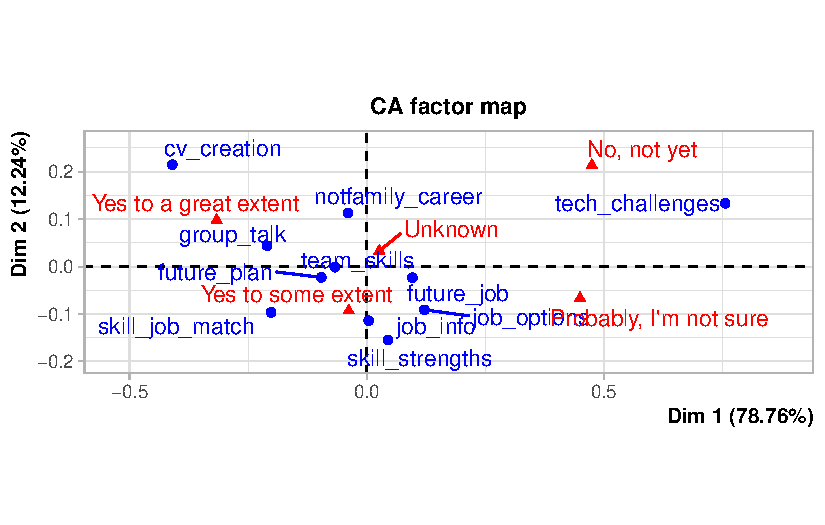
\includegraphics{Journal_article_files/figure-pdf/unnamed-chunk-7-1.pdf}

}

\end{figure}

\begin{Shaded}
\begin{Highlighting}[]
\FunctionTok{fviz\_ca\_biplot}\NormalTok{(fm2, }\AttributeTok{repel =} \ConstantTok{TRUE}\NormalTok{)}
\end{Highlighting}
\end{Shaded}

\begin{figure}[H]

{\centering 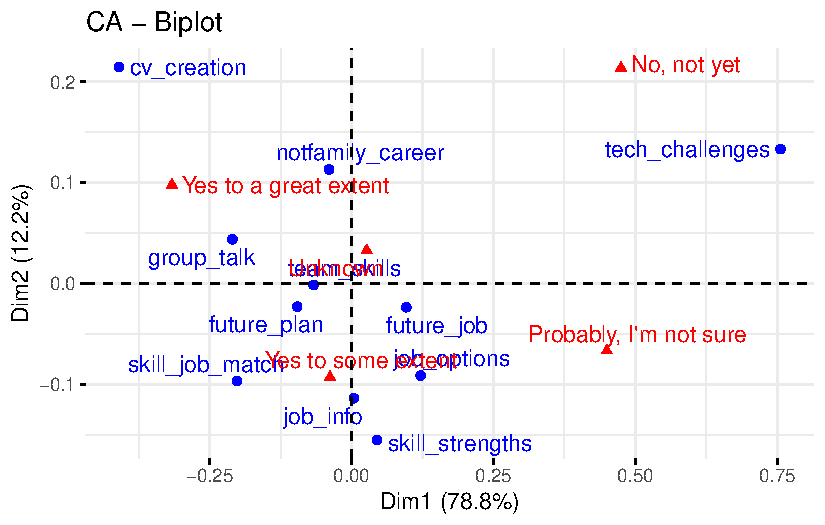
\includegraphics{Journal_article_files/figure-pdf/unnamed-chunk-8-1.pdf}

}

\end{figure}

As parametric tests may not be appropriate due to randomness issue, I
apply here chi-square test (non-parametric) to find out association
between skills and competency. The relative contribution of each cell to
the total Chi-square score give some indication of the nature of the
dependency in between rows and columns of the contingency table. This
shows that the row technological challenges, there is more who have
either no information or not sure . While `most attributes of other
variables seem independent of each other. CV creation seems highly
correlated with great extent , not aware and to some extent.

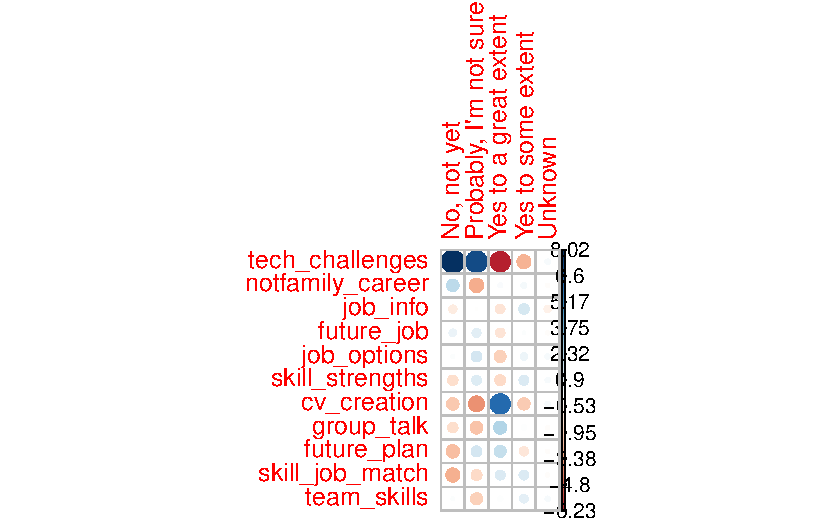
\includegraphics{Journal_article_files/figure-pdf/unnamed-chunk-9-1.pdf}

After having awareness assessment about technical, future jobs , team
skills, next set of questions were related to their strengths in certain
skills important for jobs of today and tomorrow. Following are the
tables, graphs and chi-square test regarding these atrributes.

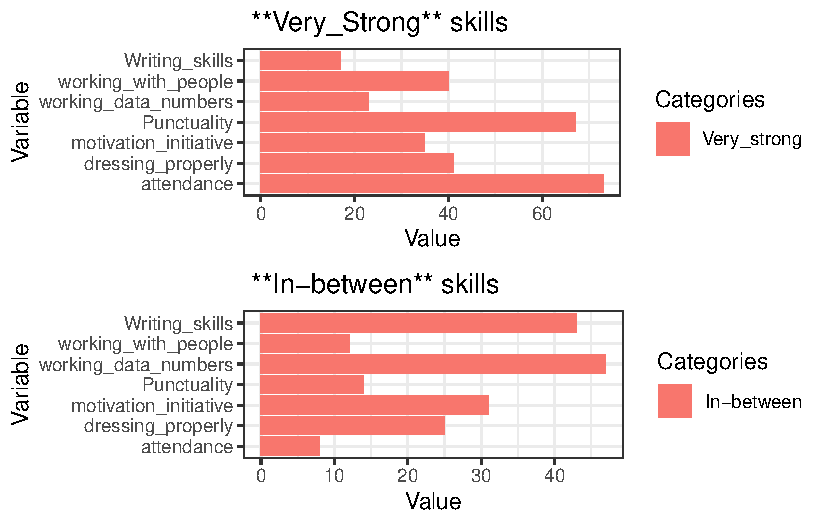
\includegraphics{Journal_article_files/figure-pdf/unnamed-chunk-11-1.pdf}

This is an exploratory analysis indicating that relatively large number
of respondents report very strong in skills like hard work and
punctuality while a large number of respondents are not very confident
and report as In\_between e.g: writing skills, working in a team,
motivation and initiative, working with data and numbers and in other
skills. There is no substitute for hard work. Nevertheless, without
smart work, it seems remote possibility that our youth can excel in
opportunities offered by jobs of today and tomorrow by simply hard. They
have to invest in soft skills. This survey was based on self reported
confidence which is usually biased upward. Caution should be observed
while generalizing these results as it is non-probability sample.

\hypertarget{career-counseling-and-support}{%
\section{Career Counseling and
Support}\label{career-counseling-and-support}}

There are lot of online learning opportunities, but many often ask that
they don't have access to trustworthy sources from where they can get an
idea from which source to learn. Unlike consumer common products used in
Pakistan, there are not many reviews about learning platforms. Some
complains that online learning/training are either below quality or fake
and charge hefty amounts to participants. Workers often ask how to make
sense of their options but there is not sufficient information available
on the matter. Potential consumers of online education encounter a black
box. Survey results from 112 university graduates indicates that they
are performing poor in studies because no right counseling was provided
to them when they join BS-graduate program. A survey mainly from entry
level graduates was conducted from students. This survey may not fulfill
criteria of random sampling, so I am not generalizing results on the
basis of statistical inference. Based on these survey results it has
been found that one of the reasons for poor performance of graduate
students during their studies is lack of mentoring and counseling to
choose the right discipline. Many of the students join a discipline
without due consideration. This hampers their opportunities to excel in
future. Following are the responses to one the question asked: Do you
think choice of degree would have been better if you were provided
career counseling before admission to a university? and Do you think
career counseling be made mandatory before joining university? \emph{Do
you think choice of degree would have been better if you were provided
career counseling before admission to a university?} and \emph{Do you
think career counseling be made mandatory before joining university?}

\begin{longtable}[]{@{}ll@{}}
\toprule()
Response & \%age \\
\midrule()
\endhead
Yes & 68.8\% \\
No & 13.4\% \\
Maybe & 17.9\% \\
& \\
\bottomrule()
\end{longtable}

\begin{center}\rule{0.5\linewidth}{0.5pt}\end{center}

\hypertarget{choice-of-degree-with-career-would-have-been-better-with-counseling}{%
\subsection{Choice of degree with career would have been better with
counseling}\label{choice-of-degree-with-career-would-have-been-better-with-counseling}}

\begin{longtable}[]{@{}
  >{\raggedright\arraybackslash}p{(\columnwidth - 2\tabcolsep) * \real{0.2778}}
  >{\raggedright\arraybackslash}p{(\columnwidth - 2\tabcolsep) * \real{0.2361}}@{}}
\caption{Should career-counseling be mandatory}\tabularnewline
\toprule()
\begin{minipage}[b]{\linewidth}\raggedright
Response
\end{minipage} & \begin{minipage}[b]{\linewidth}\raggedright
\% response \textbar{}
\end{minipage} \\
\midrule()
\endfirsthead
\toprule()
\begin{minipage}[b]{\linewidth}\raggedright
Response
\end{minipage} & \begin{minipage}[b]{\linewidth}\raggedright
\% response \textbar{}
\end{minipage} \\
\midrule()
\endhead
Strongly agree

Agree

Nuetral

Disagree

Strongly Disagree & 67.5\%

26.3\%

5.5\%

0.7\%

0\% \\
\bottomrule()
\end{longtable}

These preliminary results indicate that career counseling is one
important missing link when students decide about their degree after 12
years of education. This results not only in poor academic performance
but also becomes a hindrance in their continuous learning process which
is important for youth to prepare itself for future jobs and to become a
continuous learner to reskill/upskill. Element of mentoring, counseling,
and helping youth to make informed decisions about their careers are
some important aspects to prepare our youth for future jobs and to make
them a continuous learner rather being discouraged and dejected youth.
\#\# Free lancers earnings A nationally representative survey from
individuals, who were trained through online free lancing skills,
results are endorsing the point that in this era of Silicon valley , its
not degree but skills matter. Many undergraduate students are earning a
reasonable money through this platform of free lancing.

\begin{longtable}[]{@{}ll@{}}
\caption{Table 12 Average earnings per month in USD by
qualification}\tabularnewline
\toprule()
Qualification & Earnings (USD) \\
\midrule()
\endfirsthead
\toprule()
Qualification & Earnings (USD) \\
\midrule()
\endhead
Matric & 165.54 \\
Intermediate & 156.76 \\
Bachelor & 198.94 \\
Masters & 117.54 \\
PhDs & 350.00 \\
\bottomrule()
\end{longtable}

\hypertarget{sec-conc}{%
\section{Conclusion}\label{sec-conc}}

Exploratory data analysis results indicate that our graduates are hard
working, punctual but lacking some important soft skills required in the
job market. Most of them need right mentoring and sufficient exposure to
become continuous learner. On right mentoring, university academia has
to keep itself updated and has to guide students for right learning
resources. Regarding soft skills and developing competency among
graduates, it is important to switch from a factory forced model to
learning/problem-solving outcome university model. As \citet{Weise2020}
has rightly pointed out in her book that if ``we want to move from a
future we dont want to a future we want, we have to consciously practice
bold thinking to achieve the desired future.'' Prevailing learning
culture in universities is based on teaching students for a certain
number of years and granting a piece of paper having grades written on
it. It does not indicate learning skills of a student. Similarly, gaps
exist between learners, learning providers and employers. Neither side
understands clearly what the other sides need. Adult learners need
guidance and need mentors. Most of them are unable to move on a learning
curve at their own, therefore, they need guidance.\\
With human help, adult learners can make their online learning more
effective. Learning and upskilling alone are not enough. Codding
apprenticeship, legal services, food stamps, health care, employment
assistance Guidelines to reskilling/upskilling are not available, and it
is not possible for workers to improve their skills and once they get
out of job, they hardly find any working opportunity afterward due to
change in required skills. It is needed to shift from a factory-model
(enforced content-based learning) to interactive, engaged and
problem-solving learning ecosystem. Opinion survey results indicate that
our youth is ready to work hard but to make it work smart and tap
opportunities in global gig market economy, it must invest in skills
that helps it to work smart. Probably there is need to change a mindset
from ``Slow and steady wins the race'' to ``Smart and steady wins the
race''.

\textbf{Key recommendations}: Exposing graduates to a wide variety of
skills, mentoring them on reliable resources, strengthening soft skills
and enabling them to move on a continuous learning path. Moreover, there
is need to create opportunities for working learners for re-skilling and
up-skilling opportunities. The most effective way to impart/attain
future job skills is to focus on integrating required skills with a new
learning eco-system for our youth to have decent jobs and employers
improve their efficiency and productivity.

\hypertarget{supplementary-material}{}
\bigskip

\begin{center}

{\large\bf SUPPLEMENTARY MATERIAL}

\end{center}

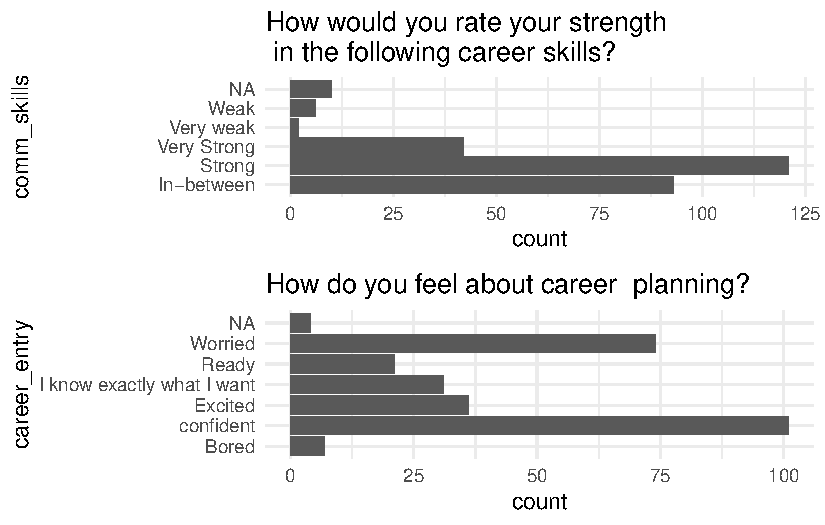
\includegraphics{Journal_article_files/figure-pdf/unnamed-chunk-16-1.pdf}

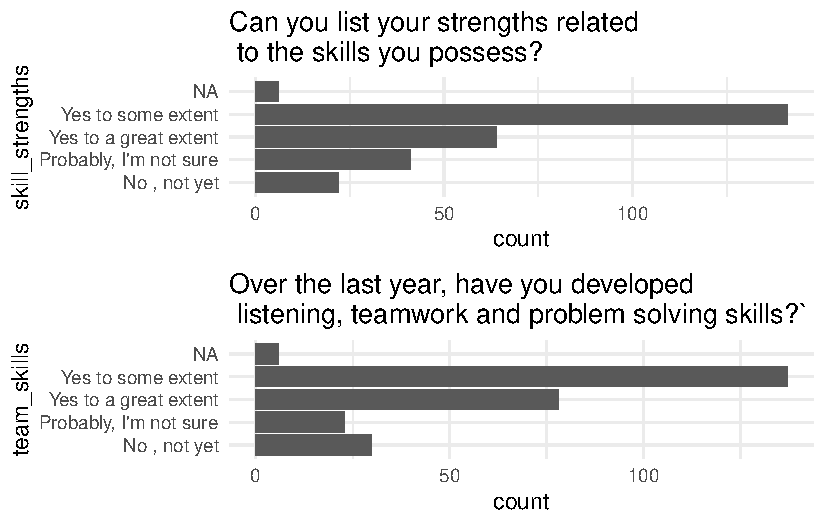
\includegraphics{Journal_article_files/figure-pdf/unnamed-chunk-16-2.pdf}

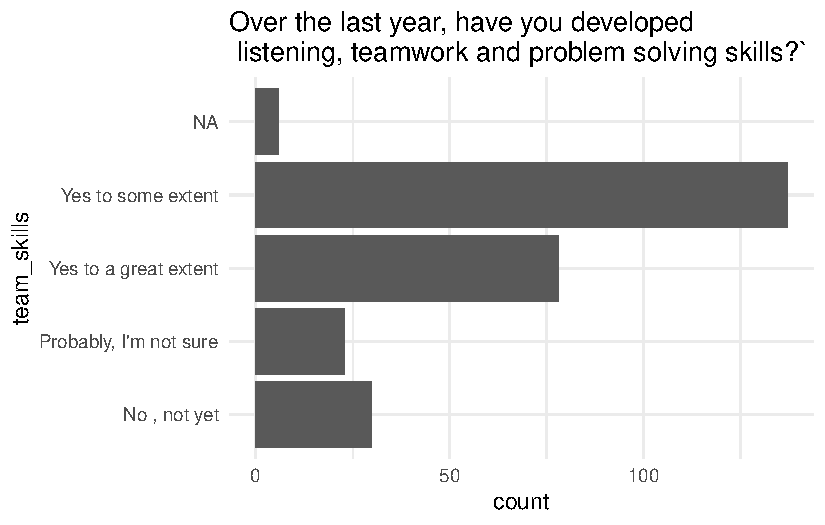
\includegraphics{Journal_article_files/figure-pdf/unnamed-chunk-16-3.pdf}


\renewcommand\refname{BibTex}
  \bibliography{bibliography.bib}


\end{document}
